\documentclass{report}
\usepackage[margin=1in, paperwidth=8.5in, paperheight=11in]{geometry}
%Math packages%
\usepackage{amsmath}
\usepackage{amsthm}
%Spacing%
\usepackage{setspace}
%Package to adjust indentation%
\usepackage{changepage}
\onehalfspacing
%Lecture number%
\newcommand{\lectureNum}{1}
%Variables - Date and Course%
\newcommand{\curDate}{February 9, 2017}
\newcommand{\course}{CS 240}
%Defining the example tag%
%\theoremstyle{definition}%
\newtheorem{ex}{Example}[section]
%Setting counter given the lecture number%
\setcounter{chapter}{\lectureNum{}}
%Package to insert code%
\usepackage{listings}
\usepackage{courier}
\usepackage{xcolor}
\lstset { 
    tabsize=2,
    breaklines=true,
    language=C++,
    backgroundcolor=\color{blue!8}, % set backgroundcolor
    basicstyle=\footnotesize\ttfamily,% basic font setting
}
%Package to draw trees%
\usepackage{tikz}
\begin{document}
%Note title%
\begin{center}
\begin{Large}
\textsc{CS 240 Midterm Review}\\
\end{Large}
Bartosz Antczak\\
\textit{Disclaimer: these questions were taken from past midterms and assignments but may not reflect what's going to be on this current midterm.}
\end{center} 

% Actual Notes%
\section*{Problem Set 1 | Runtime Notation}
\subsection{O-notation}
Show that $f(n) = 5n^3 + n^2 + 10n + 7 \in O(n^3)$.
\subsubsection{Solution:}
We must provide $n_0,\, c$ such that $\forall n \geq n_0$, $f(n) \leq cn^3$. For all $n \geq 7$
\begin{align*}
n^3 &\geq 7 \\
5n^3 &\geq 5n^3 \\
n^3 &\geq n^2 \\
10n^3 &\geq 10n \\
17n^3 &\geq f(n) && \text{(add all of the inequalities)}
\end{align*}
Choose $c = 17, \, n_0 = 7$. Thus, $f(n) \in O(n^3)$
\subsection{Big-Theta Notation}
Show that $f(n) = \frac{n^3}{n + 10} \in \Theta(n^2)$
\subsubsection{Solution:}
Provide an upper \textbf{and} lower bound:
\begin{align*}
\frac{n^3}{n + 10} \leq \frac{n^3}{n} &= n^2 \quad \forall n \geq 1 \\
\frac{n^3}{n+10} \geq \frac{n^3}{n+n} &= \frac{n^2}{2} \quad \forall n \geq 10 \\
\end{align*}
Choose $c_1 = \displaystyle \frac{1}{2}$, $c_2 = 1$, $n_0 = 10$. Thus, $f(n) \in \Theta(n^2)$.
\subsection{Recurrence}
What is the runtime of $T(n) = 2T(n-1) + 1$ with $T(1) = 1$?
\subsubsection{Solution:}
Expand this relation:
\begin{align*}
2(2T(n-2) + 1) + 1 &= 2^2 T(n-2) + 3 \\
2(2(2T(n-3) + 1) + 1) + 1 &= 2^3 T(n-3) + 5 \\ 
2(2(2(2T(n-4) + 1) + 1) + 1) + 1 &= 2^4 T(n-4) + 7 \\ 
\end{align*}
We observe a pattern. The relation is modelled as
$$2^{n-1} + \sum_{i=0}^{n-1} 2^i + 1$$
Observe that $\displaystyle \sum_{i=0}^{n-1} 2^i \in O(2^n)$ (as shown in our course notes). Thus, this recurrence relation has a runtime of $O(2^n)$.
\section*{Problem Set 2 | Loop Analysis}
\subsection{Loop 1}
What is the runtime of this algorithm?
\begin{lstlisting}
for (i = 1 to n)
	j = n^3
	while (j >= 1)
		j = j/3
\end{lstlisting}
\subsubsection{Solution:}
Observe that the while loop runs in $$\log_3(n^3) = 3\log_3(n)$$ And the outer for loop runs in
$$\sum_{i=1}^n 3\log_3(n) = 3n\log_3(n) \in O(n \log n)$$
\subsection{Loop 2}
\begin{lstlisting}
s = 1
for (i - 1 to n^2)
	for (j = 1 to n^3)
		for (k = 1 to j)
			s = 2 * s
\end{lstlisting}
\subsubsection{Solution:}
Focusing on the first two inner-most loops, the runtime is structured as
$$\sum_{j=1}^{n^3}\left(\sum_{k=1}^j 1\right) = \sum_{j=1}^{n^3} j = \frac{n^3(n^3 + 1)}{2}$$
Analysing the outer loop, it has a runtime of
$$\sum_{i=1}^{n^2} \frac{n^3(n^3 + 1)}{2} \in O(n^8) $$
Therefore, the algorithm has a runtime of $O(n^8)$.
\section*{Problem Set 3 | Heaps}
Let $n = 2^k - 1$. Write an algorithm that merges two heaps, $T_1, T_2$, both of size $n$, in $o(n)$.
\subsubsection{Solution:}
Observe that both of the heaps are full (since their size is $2^k - 1$, and by the structural property of heaps, every level must be filled). Our approach is as follows:
\begin{enumerate}
\item Take $x$, the smallest node in in $T_2$, and make it a new root, where its left and right children are $T_1$ and $T_2$ respectively.
\item Bubble down on $x$.
\end{enumerate}
The visual representation of the new heap created is shown:
\begin{figure}[ht]
\begin{center}
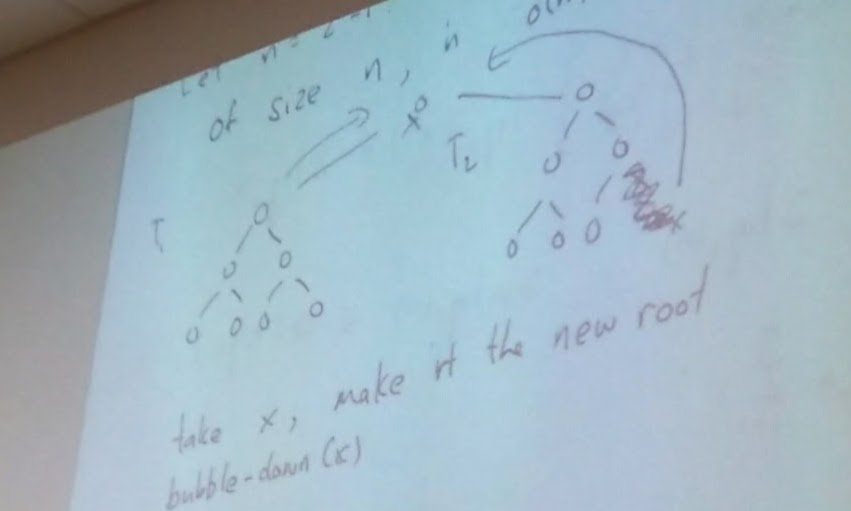
\includegraphics[scale=0.35]{heap1.jpg}
\end{center}
\end{figure}\\
This process has a runtime of $\log (n) \in o(n)$, as required.
\section*{Problem Set 4 | Tries}
Suppose we have a set of strings (hex numbers) $X = \{x_1, \cdots, x_n\}$, where $x_i < t$. If we store $x$ in a compressed trie,
\begin{itemize}
\item[a)] What is the space needed?
\subsubsection{Solution:}
Similar to how every node in a trie containing binary numbers will have \textbf{2} children, every node in this hexadecimal trie will have at most \textbf{16} children. For $n$ leaves in the trie, the total number of internal nodes is $n-1$. So, the internal nodes require $16(n-1)$ amount of space, and the leaves require $dn$ amount of space (where $d$ is a constant). In total, the amount of memory required is
$$16(n-1) + dn \in O(n)$$
Thus, we need $O(n)$ amount of space.
\item[b)] What is the height?
\subsubsection{Solution:}
The height is $O(\log_{16} (t))$
\end{itemize}
\section*{Problem Set 5 - Randomized Algorithms}
Given the randomized algorithm, which finds the minimum value of an array $A$ of size $n$:
\begin{lstlisting}
find-min(A)
	i = random(n) // O(1)
	if (min(A, i)) // O(n)
		return A[i] // O(1)
	else
		return find-min(A) // O(?)
\end{lstlisting}
Find the best-case, worst-case, and expected-case.
\subsubsection{Solution:}
\begin{itemize}
\item \textbf{Best-case:} the first randomly generated number is the correct index, so we never recurse, which results in $O(n)$
\item \textbf{Worst-case:} we never generate the correct index number, so the algorithm does not terminate
\item \textbf{Expected Case:} let $T(n)$ be the expected runtime. By definition (and also from our course notes),$$T(n) = \sum_n \mathrm{Pr}(n) \cdot n$$
Solving the equation, we get
\begin{align*}
T(n) &= \frac{1}{n}(cn) + \frac{n-1}{n}\left(T(n) + cn\right) \\
nT(n) &= nc + (n-1)T(n) + nc(n-1) && \text{(Doing some algebra)} \\
T(n) &= 2(n-1)nc \in O(n^2)
\end{align*}
Therefore, the expected runtime is $O(n^2)$.
\end{itemize}
\begin{center}
\textit{Best of luck on the midterm! :)}
\end{center}
%END%
\end{document}